
\section{Track A: The Full-Corpus Attempt Campaign}
\label{sec:tracka}

Track A is the estate's flagship honesty instrument: an automated campaign that attempts \emph{every} declaration in the Lean corpus's attempt scope and records the outcome of each attempt as an immutable receipt --- including failures. The campaign ran to completion on November 14--15, 2026:

\begin{itemize}
\item \textbf{143 of 143} declarations attempted (full coverage, no silent skips);
\item \textbf{65} attempts echoed \texttt{sorry} (the tactic emits \texttt{sorry} when it cannot close the goal: an honest failure, recorded as such);
\item \textbf{0} attempts returned empty output;
\item \textbf{0} attempts were recorded as fabrications (no attempt was credited without a kernel-checked or explicitly failed trace).
\end{itemize}

The campaign ran in two recorded stages. Stage one halted at its target of 44 declarations --- the halt itself recorded in the campaign receipt rather than smoothed into the headline --- and stage two (the resumed full-corpus pass, campaign close \texttt{CAMPAIGN2\_DONE}, 03:39:38Z, November 15) attempted the remaining 100 declarations, of which 65 echoed \texttt{sorry}. The two stages sum to the 143-attempt denominator; Table~\ref{tab:stages} gives the per-stage accounting.

\begin{table}[htbp]
\centering
\small
\begin{tabular}{lrrr}
\toprule
\textbf{Stage} & \textbf{Attempted} & \textbf{Echoed \texttt{sorry}} & \textbf{Empty / fabricated} \\
\midrule
Stage 1 (halted at target 44) & 43 & recorded per-receipt & 0 / 0 \\
Stage 2 (\texttt{CAMPAIGN2\_DONE} 03:39:38Z) & 100 & 65 & 0 / 0 \\
\midrule
\textbf{Total} & \textbf{143} & \textbf{per-receipt} & \textbf{0 / 0} \\
\bottomrule
\end{tabular}
\caption{Track A per-stage accounting. The stage-one halt at its target is recorded, not hidden; the stage-two close receipt carries the echoed-\texttt{sorry} count.}
\label{tab:stages}
\end{table} All 143 attempt receipts are published in the dataset \texttt{SZLHOLDINGS/lean-proof-corpus-v1} under \texttt{receipts/track\_a\_attempts/}, and were re-verified against the dataset tree API after the campaign closed (143 files present, byte-verified against the local manifest). Figure~\ref{fig:tracka} shows the outcome distribution.

\begin{figure}[htbp]
\centering
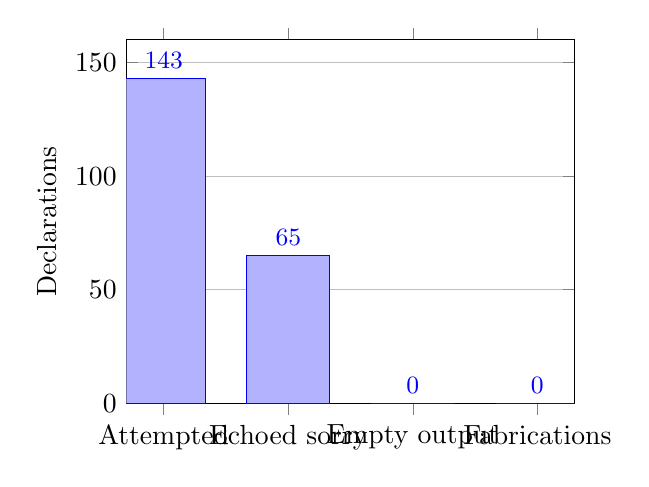
\begin{tikzpicture}
\begin{axis}[
  ybar, bar width=30pt,
  width=0.6\textwidth, height=6.2cm,
  symbolic x coords={Attempted, Echoed sorry, Empty output, Fabrications},
  xtick=data, ymin=0, ymax=160,
  ylabel={Declarations},
  nodes near coords, every node near coord/.append style={font=\small},
  ymajorgrids=true,
]
\addplot coordinates {(Attempted,143) (Echoed sorry,65) (Empty output,0) (Fabrications,0)};
\end{axis}
\end{tikzpicture}
\caption{Track A full-corpus campaign outcomes (November 14--15, 2026). The 65 \texttt{sorry}-echo failures are the point: a corpus whose failure mode is visible is a corpus whose successes mean something.}
\label{fig:tracka}
\end{figure}

\paragraph{Why report failures as headline results.} A proof-assistant campaign that reports only closed goals invites the suspicion that the denominator was chosen after the numerator. Track A fixes the denominator first (every declaration in scope), then reports the numerator honestly. The 45.5\% closure rate implied by the complement of the \texttt{sorry} echo is a \emph{real} number only in the sense that it is bound to a fixed scope and reproducible; the estate makes no comparative claim against external corpora, whose scopes differ.

\section{The Evaluation Battery}
\label{sec:battery}

The evaluation battery binds models to fixed six-item benchmark batteries and records per-binding scores in commit-addressed logs. Two waves are reported; both are published in full.

\subsection{Wave 4 (bind-31)}
The wave-4 binding log records 35 binding entries: \textbf{24} bindings scored \textbf{3/6}, \textbf{7} scored \textbf{4/6}, and the remaining \textbf{4} entries carry other or unrecorded scores (each visible as its own line in the log, none silently dropped). No binding exceeded 4/6.

\subsection{Battery v5 era}
The most recent binding log (the \texttt{bind\_battery\_log.jsonl} of the v5 battery era) records 41 bindings: \textbf{37} scored \textbf{0/6}, \textbf{3} scored \textbf{3/6}, \textbf{1} scored \textbf{4/6}. The modal score is zero. Figure~\ref{fig:battery} shows both waves.

\begin{figure}[htbp]
\centering
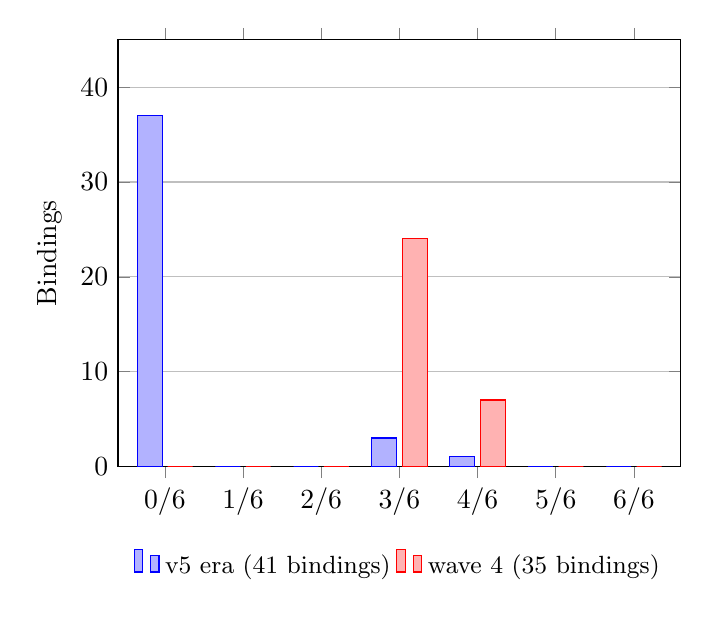
\begin{tikzpicture}
\begin{axis}[
  ybar, bar width=9pt,
  width=0.72\textwidth, height=7.0cm,
  symbolic x coords={0/6, 1/6, 2/6, 3/6, 4/6, 5/6, 6/6},
  xtick=data, ymin=0, ymax=45,
  ylabel={Bindings},
  legend style={at={(0.5,-0.18)}, anchor=north, legend columns=2, font=\small, draw=none},
  ymajorgrids=true,
]
\addplot coordinates {(0/6,37) (1/6,0) (2/6,0) (3/6,3) (4/6,1) (5/6,0) (6/6,0)};
\addplot coordinates {(0/6,0) (1/6,0) (2/6,0) (3/6,24) (4/6,7) (5/6,0) (6/6,0)};
\legend{v5 era (41 bindings), wave 4 (35 bindings)}
\end{axis}
\end{tikzpicture}
\caption{Evaluation battery score distributions, both published waves, November 2026. The v5-era mode at 0/6 (37 of 41) is the headline: the battery binds harder instruments and most bindings abstain. Wave 4's four unrecorded-score entries are excluded from its bars and remain visible in the raw log.}
\label{fig:battery}
\end{figure}

\paragraph{Log integrity.} Each binding entry is written with content-addressed verification: the binding is written, read back, and its digest logged; the log files themselves are mirrored to the receipt datasets after each wave. The two waves reported here are therefore re-readable in full, entry by entry --- including the entries that score zero and the four unrecorded wave-4 entries, which are visible as their own lines rather than dropped.

\paragraph{The 0/6 wave is the finding.} The v5-era log is dominated by 0/6 scores because the battery's v5 instruments are abstention-heavy: the evaluated bindings, when they cannot answer an item, emit an abstention that scores as zero rather than guessing. The estate reports this distribution without smoothing because it is the direct measurement of the battery's refusal discipline. A guessing policy would produce a smoother, higher distribution --- and a dishonest one.
